% Figure 1: schematic of the diagnostic calibration (initial states, diagnostic step, Bayesian inference).
% Compile with pdflatex (standalone class; needs the packages tikz and pgfplots).
\documentclass[tikz,border=2mm]{standalone}
\usepackage{amsmath,amssymb,bm}
\usepackage{pgfplots}
\usetikzlibrary{arrows.meta, positioning, decorations.pathreplacing,fit}
\pgfplotsset{compat=1.17}

\begin{document}
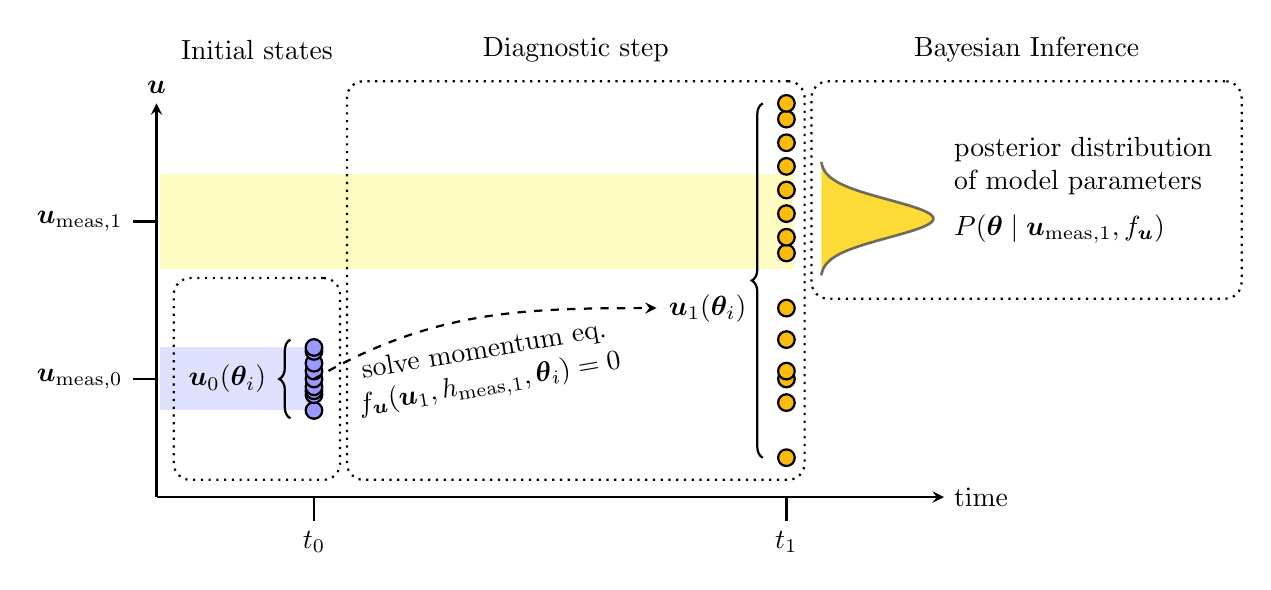
\begin{tikzpicture}[>=stealth, thick]

% Axes
\draw[->] (0,0) -- (10,0) node[right] {time};
\draw[->] (0,0) -- (0,5) node[above] {${\bm u}$};

% Time markers
\draw[thick] (2,0) -- (2,-0.3) node[below] {$t_0$};
\draw[thick] (8,0) -- (8,-0.3) node[below] {$t_1$};

% Measurements u_meas(t0), u_meas(t1)
\draw[thick] (0,1.5) -- (-0.3,1.5) node[left] {${\bm u}_{\text{meas},0}$};
\draw[thick] (0,3.5) -- (-0.3,3.5) node[left] {${\bm u}_{\text{meas},1}$};

% Shaded bands for uncertainty
\fill[blue!20,opacity=0.6] (0.05,1.1) rectangle (2,1.9);
\fill[yellow!40,opacity=0.6] (0.05,2.9) rectangle (8.1,4.1);

% Initial samples at t0 (red)
\foreach \y in {1.1,1.3,1.35,1.4,1.5,1.6,1.7,1.85,1.9}{
    \fill[blue!40!white, draw=black](2,\y) circle (3pt);
}
\node at (0.9,1.5) {${\bm u}_0({\bm \theta}_{i})$};

% Final samples at t1 (orange, larger spread including outside yellow band)
\foreach \y in {0.5,1.2,1.5,1.6, 2,2.4,3.1,3.3,3.6,3.9,4.2,4.5,4.8,5.0}{
    \fill[yellow!50!orange, draw=black] (8,\y) circle (3pt);
}
\node at (7,2.4) {${\bm u}_1({\bm \theta}_{i})$};

% Curved dashed arrow from a sample at t0 to a sample at t1
\draw[dashed,->,thick] (2,1.5) to[out=30,in=180] node[midway,below=4pt,sloped,align=center] {solve momentum eq. \\ $f_{\bm u}({\bm u}_1,h_{{\rm meas},1},{\bm \theta}_i)=0$} (6.35,2.4);

% Braces
\draw [decorate,decoration={brace,amplitude=4pt}] (1.7,1) -- (1.7,2);
\draw [decorate,decoration={brace,amplitude=4pt}] (7.7,0.5) -- (7.7,5);

% Gaussian posterior distribution (aligned with yellow band)
\begin{scope}[shift={(8.3,4.4)}, rotate=270, scale=1.2] % center at y=4
  \begin{axis}[
      hide axis,
      domain=-3:3,
      samples=100,
      width=3cm,
      height=2cm, % matches yellow band vertical extent
      axis y line=none,
      axis x line=none,
      y=1.2cm,
      x=0.2cm,
  ]
    \addplot[thick, white!30!black, fill=yellow!70!orange, opacity=0.8]
    {exp(-x^2/2)} ;%\closedcycle;
  \end{axis}
\end{scope}

% Posterior text
\node[right, align=left] at (10,4.2) {posterior distribution \\ of model parameters};
\node[right] at (10,3.4) {$P({\bm \theta} \mid {\bm u}_{{\rm meas},1},f_{\bm u})$};

% Box around Gaussian distribution
\node[draw, rounded corners=6pt, dotted, thick, inner sep=8pt, fit={(8.6,2.8) (13.5,5)}] (gaussbox) {};
\node[above=3pt of gaussbox, align=center] {Bayesian Inference};

\node[draw, rounded corners=6pt, dotted, thick, inner sep=8pt, fit={(2.7,0.5) (7.95,5)}] (gaussbox2) {};
\node[above=3pt of gaussbox2, align=center] {Diagnostic step};

\node[draw, rounded corners=6pt, dotted, thick, inner sep=8pt, fit={(0.5,0.5) (2.05,2.5)}] (gaussbox3) {};
\node[above=75pt of gaussbox3, align=center] {Initial states};


\end{tikzpicture}
\end{document}
